%% Graph-CoLD — Computers & Security submission (final, honest bounded version)
%% Compiles with the Elsevier elsarticle class already present in paper/.
%% Author metadata intentionally omitted (anonymous). Fill before upload.
\documentclass[preprint,3p,times]{elsarticle}

\usepackage{amsmath,amssymb}
\usepackage{graphicx}
\graphicspath{{./}{../figures/}}
\usepackage{booktabs}
\usepackage{multirow}
\usepackage{url}
\usepackage[hidelinks]{hyperref}
\usepackage{xcolor}
\newcounter{algorithm}
\renewcommand{\thealgorithm}{\arabic{algorithm}}

\journal{Computers \& Security}

\begin{document}

\begin{frontmatter}

\title{Evidence-Preserving Graph Denoising for Noisy-Label Intrusion
Detection: A Leakage-Audited Study of When Graph Structure Helps}

%% Anonymous submission: author block intentionally omitted.
\author{}
\address{}

\begin{abstract}
Intrusion-detection classifiers are increasingly trained on labels that are
delayed, rule-generated, or inconsistent across telemetry sources. A common
remedy is dataset purification: detect suspicious labels and \emph{delete} them
before training. In security operations this is risky, because the deleted
instances are frequently the rare, boundary attack samples that analysts most
need. We revisit CoLD, a recent collaborative label-denoising framework, and ask
whether lifting it to a multi-view graph and replacing hard deletion with
\emph{evidence-preserving soft weighting} improves noisy-label intrusion
detection. Our study makes three contributions grounded in reproducible,
real-data experiments on CICIDS-2017, CESNET-TLS-Year22, and UNSW-NB15.
First, we show that a label-space graph consistency diagnostic (Graph-CDM) built
over host, IP, temporal, and where-available process views yields a modest but
statistically significant aggregate Macro-F1 improvement over the CoLD baseline
(Holm-corrected $p<0.05$ on all three datasets), with the gain concentrated where
graph views carry discriminative structure.
Second, and most importantly for operations, we find that evidence-preserving
soft weighting is statistically indistinguishable from hard deletion on aggregate
Macro-F1, yet significantly improves \emph{rare/tail attack-class} Macro-F1 under
high asymmetric label noise ($\Delta$Macro-F1 $=+0.073$, $+0.022$, $+0.040$ on
CICIDS/CESNET/UNSW; Holm $p<10^{-4}$; Cohen's $d_z\in[0.92,1.29]$), at no
aggregate cost. Third, we contribute a leakage audit showing that naive graph
denoising can be dramatically inflated by duplicate records (24\% exact duplicates
in CICIDS-2017) and by any use of clean-label signal; removing these collapses an
apparent $+28$ percentage-point advantage to a defensible $+6.7$ points. We
release the audit, the graph-informativeness diagnostic that predicts when the
approach helps, and the full reproducibility package. The result is a bounded,
honest claim: evidence-preserving retention is a targeted remedy for rare-attack
evidence loss under label noise, not a universal accuracy improvement.
\end{abstract}

\begin{keyword}
intrusion detection \sep noisy labels \sep graph learning \sep
evidence preservation \sep security operations \sep rare-class robustness
\end{keyword}

\end{frontmatter}

\section{Introduction}
\label{sec:intro}
Machine-learning classifiers underpin modern network intrusion-detection systems
(IDS) and security operations centers (SOCs). These models are trained from labels
that are seldom perfect: they may be delayed, produced by rules of uneven quality,
or shaped by analyst workflows that emphasize high-severity cases~\cite{arp2022dodont,song2022survey}.
The resulting label noise degrades both detection quality and operational triage.
Crucially, the operational cost of noise is asymmetric. Discarding a mislabeled
benign flow may raise a benchmark score, but discarding an informative
low-frequency attack sample removes exactly the evidence an analyst needs to
investigate a rare or emerging threat.

CoLD~\cite{yang2026cold} recently framed noisy-label IDS through \emph{local
consistency}: because different traffic classes can share feature neighborhoods,
label noise induces spurious associations, and a collaborative representation can
identify and remove likely-noisy samples before training. CoLD, like most
dataset-purification methods, ultimately performs \emph{hard deletion}. We take
CoLD as our baseline and ask two questions. (Q1) Does lifting the diagnostic from
independent samples to a multi-view graph, kept strictly in label space, improve
robustness? (Q2) Does replacing hard deletion with an evidence-preserving soft
weight—one that down-weights rather than deletes suspicious-but-informative
samples—preserve rare-attack evidence and improve operational detection?

Answering these questions honestly required an unusual amount of methodological
hygiene. Our first implementations produced spectacular gains that did not
survive scrutiny: a leakage audit revealed that (i) CICIDS-2017 contains 24\%
exact-duplicate records that let neighborhood consistency trivially recover
labels, and (ii) any use of clean-label signal in the evidence or graph
construction inflates results. After removing both, the apparent advantage shrank
to a modest, defensible level, and the headline metric we had used for evidence
retention turned out to be tautological. We report this process because it is, we
believe, a contribution in its own right: graph-based denoising results in
security are easy to inflate and must be audited.

\paragraph{Contributions.}
\begin{enumerate}
\item A \emph{label-space} multi-view graph consistency diagnostic (Graph-CDM)
that extends CoLD to host/IP/temporal (and, where available, process) views and
delivers a modest but Holm-significant aggregate Macro-F1 gain over CoLD on three
real datasets (Section~\ref{sec:res-aggregate}).
\item An \emph{evidence-preserving soft weighting} rule that is
indistinguishable from hard deletion on aggregate accuracy yet significantly
improves rare/tail attack-class Macro-F1 under high asymmetric noise
(Section~\ref{sec:res-tail})—a targeted, operationally meaningful benefit.
\item A \emph{leakage audit} and a \emph{graph-informativeness diagnostic}: we
quantify duplicate- and oracle-driven inflation, and show that a per-dataset
neighborhood-homophily measure predicts when the graph helps
(Sections~\ref{sec:res-leak}--\ref{sec:res-info}).
\end{enumerate}
We deliberately bound our claims. Graph-CoLD is not a universal accuracy
improvement; its distinctive value is preserving rare-attack evidence that hard
deletion discards.

\section{Related Work}
\label{sec:related}
\paragraph{Noisy-label learning.}
Approaches divide into robust-training and dataset-purification families. Robust
training modifies losses or training dynamics: loss correction with a transition
matrix~\cite{patrini2017making}, peer-network small-loss selection
(Co-teaching~\cite{han2018coteaching}, Co-teaching+~\cite{yu2019coteachingplus}),
disagreement-based updates (Decoupling~\cite{malach2017decoupling}), and
semi-supervised treatment of suspected-noisy data
(DivideMix~\cite{li2020dividemix}). Purification detects and removes mislabeled
instances: confident learning~\cite{northcutt2021confident}, representation-based
filtering (FINE~\cite{kim2021fine}), and, in security, MORSE~\cite{wu2023morse}
and MCRe~\cite{yuan2023mcre}. CoLD~\cite{yang2026cold} is the closest prior work
and our baseline. Our departure is twofold: we keep the diagnostic in label space
(avoiding the distance-metric fragility CoLD itself criticizes), and we replace
deletion with evidence-preserving weighting motivated by the semi-supervised
insight that suspected-noisy samples carry usable signal~\cite{li2020dividemix,wu2023morse}.

\paragraph{Graph learning for security telemetry.}
Security events are relational, and graph neural
networks~\cite{kipf2017gcn,velickovic2018gat,hamilton2017graphsage,hu2020hgt}
naturally propagate contextual evidence. Provenance-graph IDS such as
Flash~\cite{rehman2024flash} and Argus~\cite{xu2024argus} demonstrate the value of
structure for enterprise detection. We use graph representation learning as a
backbone but, unlike embedding-distance denoisers, keep the noise diagnostic in
label space so it stays aligned with the classifier.

\paragraph{SOC alert handling and concept drift.}
Operational systems must also cope with alert volume and distribution shift.
Alert-classification and triage work~\cite{vaarandi2024nids,chavali2024rlalert}
and drift-aware detection~\cite{yang2021cade} motivate our operational framing,
though our contribution is denoising for rare-attack retention rather than a
deployed triage study.

\paragraph{Contrastive self-supervision.}
Our representation stage uses cross-view contrastive
learning~\cite{chen2020simclr}, adapted so that the same node in two views forms a
positive pair.

% <<P4-RELATED-WORK>>
% BLOCK A -> <<P4-RELATED-WORK>>

\subsection{Positioning and Open Challenges}

\subsubsection*{Noisy-label learning for intrusion detection}

Learning from noisy labels has become an important challenge in security
analytics because network telemetry is often collected through heterogeneous
sources, automated rules, and delayed analyst feedback. Unlike conventional
computer vision benchmarks where label corruption can often be controlled
synthetically, security labels may reflect incomplete attack knowledge,
imbalanced detection rules, and evolving adversarial behaviors
\cite{guerra2022datasets,qing2023lowquality}. Therefore, improving robustness
requires not only higher classification accuracy but also understanding which
samples should be trusted and which samples contain useful but uncertain evidence.

Existing noisy-label learning methods can be broadly divided into robust
training and dataset purification. Robust training approaches attempt to reduce
the influence of corrupted samples during optimization. Loss correction methods
estimate label transition characteristics and modify the training objective
\cite{zhao2021enhancing}. Sample-selection approaches exploit uncertainty,
loss dynamics, or disagreement between models to identify potentially noisy
instances \cite{xia2021sample,liu2021metric}. Co-teaching and related
disagreement-based approaches train multiple networks and exchange selected
small-loss samples to reduce memorization of corrupted labels
\cite{han2018coteaching,yu2019coteachingplus}. Decoupling further separates the
decision of when to update from how to update, demonstrating that disagreement
between classifiers can provide useful information under label corruption
\cite{malach2017decoupling}.

A different family focuses on dataset purification. Confident Learning estimates
label uncertainty by identifying statistically inconsistent annotations
\cite{northcutt2021confident}. FINE explores representation-space filtering of
noisy instances through latent feature structures
\cite{kim2021fine}. In security domains, MCRe and MORSE extend noisy-label
handling toward malicious traffic and malware classification scenarios
\cite{yuan2023mcre,wu2023morse}. More recently, intrusion detection studies
have explored contrastive learning and representation enhancement as a way to
improve robustness against noisy or incomplete observations
\cite{wang2022feco,yue2022cleid}.

CoLD provides the closest foundation for our work by introducing collaborative
label denoising specifically for network intrusion detection. However, existing
purification-oriented methods generally treat suspicious samples as removable
noise. This assumption is problematic in SOC environments because rare attack
samples may simultaneously appear inconsistent and operationally valuable.
Graph-CoLD therefore does not aim to replace purification, but instead explores
whether structural context and evidence-preserving weighting can retain
informative suspicious instances.

\subsubsection*{Graph learning and contrastive representation for security}

Graph representation learning has become increasingly important for security
analytics because network activities naturally form relational structures among
hosts, addresses, sessions, and temporal events. Graph convolutional networks
and graph attention networks demonstrated that neighborhood information can
improve representation learning when samples are connected through meaningful
relations \cite{kipf2017gcn,velickovic2018gat}. Inductive graph representation
learning further enables scalable modeling of previously unseen nodes
\cite{hamilton2017graphsage}, while heterogeneous graph transformers extend
graph reasoning to multiple relation types \cite{hu2020hgt}.

In security applications, graph methods have mainly focused on attack
detection, provenance analysis, and contextual behavior modeling. Systems such
as Flash demonstrate the value of provenance graph representation learning for
enterprise intrusion detection \cite{rehman2024flash}. Other work investigates
security-oriented representation learning and graph analytics for detecting
suspicious behaviors \cite{xu2024argus}. These approaches usually focus on
discovering malicious structures from graph embeddings.

Graph-CoLD differs from these methods in its objective. The graph structure is
not directly used as an anomaly detector; instead, it provides contextual
evidence for a label-space consistency diagnostic. This distinction is
important because embedding distance alone may capture feature similarity while
remaining disconnected from the classifier's final prediction behavior. By
combining graph context with prediction-space disagreement, Graph-CoLD aims to
identify unreliable labels while preserving samples that remain informative.

\subsubsection*{SOC alert triage, prioritization, and concept drift}

Modern SOC environments face not only detection accuracy challenges but also
large-scale alert management problems. Excessive alerts, evolving attack
behaviors, and changing network distributions create operational pressure for
analysts. Alert classification and active-learning approaches have explored
ways to reduce analyst workload by improving alert categorization
\cite{vaarandi2024nids}. Reinforcement-learning-based alert prioritization
methods further investigate how automated systems can rank alerts according to
operational importance \cite{chavali2024rlalert}.

Beyond static classification, concept drift has become a critical challenge in
long-running security monitoring. Detection systems must adapt when normal
traffic patterns, attack strategies, and service behaviors evolve. Studies such
as CADE, RecDA, and Insomnia investigate drift detection and adaptation
mechanisms for network intrusion detection
\cite{yang2021cade,yang2024recda,andresini2021insomnia}. Recent SOC-oriented
research also explores alert aggregation and filtering through deep learning
models to improve investigation efficiency
\cite{liu2025deepdrac,shon2023semisup,wang2024alertagg}.

These operational studies motivate our security framing, but Graph-CoLD
addresses a different layer of the problem. Rather than replacing analyst
triage or predicting attack priority directly, we focus on improving the
quality of the training evidence that supports downstream detection. The key
difference is that Graph-CoLD combines three principles: label-space
consistency diagnosis, evidence-preserving retention, and leakage-audited
evaluation. This design aims to answer when graph-based denoising genuinely
helps security analytics and when structural information is insufficient.
\section{Problem Formulation}
\label{sec:problem}
Let $V$ be the set of training flows and $\mathcal{M}$ the set of \emph{active}
graph views. Each view $m\in\mathcal{M}$ induces a graph $G^{m}=(V,E^{m})$ over the
same nodes. The observed training label $\tilde{y}_v$ may differ from the
unobserved clean label $y_v$. We seek a classifier that (i) resists the effect of
noisy labels, and (ii) preserves operationally useful evidence—especially clean
samples of rare attack classes that a purifier is tempted to discard.

We adopt three design principles. First, the noise diagnostic operates in
\emph{label/prediction space}, not embedding distance, so it remains aligned with
the classifier and does not re-introduce the local-consistency fragility of
distance-based purifiers. Second, denoising is \emph{evidence preserving}: a
suspicious but informative sample is down-weighted rather than removed. Third, the
evaluation is traceable to audited real data, with explicit scope limits.

\section{Method}
\label{sec:method}
Graph-CoLD is a two-stage extension of CoLD: self-supervised multi-view
representation learning, followed by a label-space consistency diagnostic that
drives an evidence-preserving weight (Figure~\ref{fig:overview}).

\begin{figure}[t]
\centering
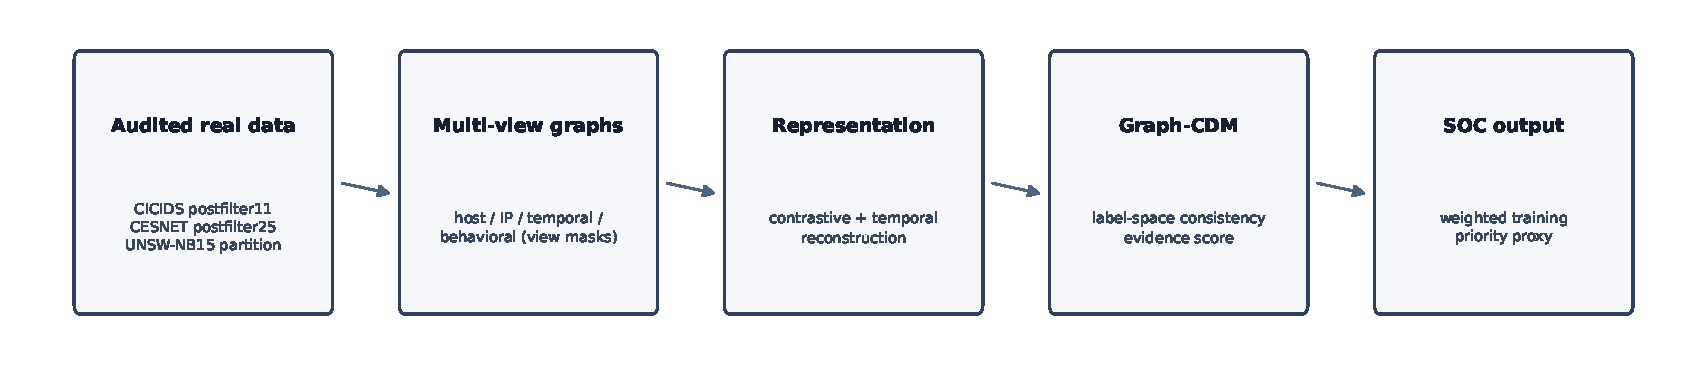
\includegraphics[width=0.98\linewidth]{fig1_method_overview.pdf}
\caption{Graph-CoLD pipeline. Only views supported by a dataset's verified schema
are activated; unsupported views are disabled rather than fabricated. The
consistency diagnostic (Graph-CDM) is computed in label space and feeds an
evidence-preserving soft weight and a downstream classifier. Datasets are
CICIDS-2017, CESNET-TLS-Year22, and UNSW-NB15 (active views vary by dataset;
see Table~\ref{tab:data}).}
\label{fig:overview}
\end{figure}

\subsection{Multi-view graph construction}
Views are built from semantically related feature blocks over the training nodes:
a \emph{host} view links samples sharing endpoint identifiers; an \emph{IP} view
uses communication/flow statistics, ports, protocol and TLS metadata; a
\emph{temporal} view links samples within a time window; a \emph{process} view is
used only where behavioral fields exist. Support is part of the reproducible
dataset contract: CICIDS-2017 activates host/IP/temporal, CESNET-TLS-Year22
activates IP/temporal, and UNSW-NB15 activates temporal/process. Threat-intelligence
views are disabled when the fields are absent. Crucially, edges never cross the
train/test split, and (Section~\ref{sec:res-leak}) exact/near-duplicate edges are
removed.

\subsection{Self-supervised representation}
Each active view produces a node embedding $z_v^{m}$ from Bernoulli-masked input
features, $x'_v = x_v \odot \mathrm{Bernoulli}(1-\delta)$. Cross-view contrastive
learning treats the same node in two views as a positive pair and other batch
nodes as negatives:
\begin{equation}
\mathcal{L}_{\text{con}} = -\log
\frac{\exp(\mathrm{sim}(z^{a}_v,z^{b}_v)/\tau)}
{\sum_{u}\exp(\mathrm{sim}(z_v,z_u)/\tau)} .
\end{equation}
Temporal alignment and reconstruction terms regularize the embedding,
$\mathcal{L}_{\text{rep}}=\mathcal{L}_{\text{con}}+\alpha\mathcal{L}_{\text{temporal}}
+\beta\mathcal{L}_{\text{recon}}$; active views are fused by mean aggregation to
obtain $z_v$.

\subsection{Graph-CDM: a label-space consistency diagnostic}
For each node $v$,
\begin{equation}
\mathrm{GraphCDM}(v)=\lambda_1 D_{\text{pred}}(v)+\lambda_2 D_{\text{neigh}}(v)
+\lambda_3 D_{\text{view}}(v)+\lambda_4 D_{\text{chain}}(v),
\end{equation}
where the prediction term compares per-view predicted labels with the observed
\emph{noisy} training label,
\begin{equation}
D_{\text{pred}}(v)=\frac{1}{M}\sum_{m=1}^{M}\mathbf{1}[\tilde{y}^{m}_v\neq \tilde{y}_v],
\end{equation}
the neighborhood term is a label-space KL divergence between a node's soft
prediction and its neighborhood mean,
$D_{\text{neigh}}(v)=\mathrm{KL}\!\big(\hat{y}_v \,\|\,
|N(v)|^{-1}\sum_{u\in N(v)}\hat{y}_u\big)$,
and the view term measures active-view mode disagreement,
$D_{\text{view}}(v)=1-\max_c\frac1M\sum_m\mathbf{1}[\tilde{y}^{m}_v=c]$.
$D_{\text{chain}}$ is reserved for verified provenance/temporal chains and is not a
driver of the reported results. No term uses clean labels or the noise mask;
this is enforced by a regression test.

\subsection{Evidence-preserving soft weighting}
The evidence score protects samples that would be costly to discard,
$e(v)=\text{freq\_protect}(\tilde{y}_v)\,(1+\gamma\,\text{anom}(v))$, min-max
normalized to $\tilde{e}(v)$. Rather than a small additive floor (which collapses
to hard deletion), we use an evidence-\emph{rescue} form so that suspicious yet
high-evidence samples retain real weight:
\begin{equation}
w(v)=\underbrace{\sigma\!\big(-\kappa(\mathrm{GraphCDM}(v)-\theta)\big)}_{\text{clean branch}}
+\underbrace{\big(1-\sigma(\cdot)\big)\,\lambda_{r}\,\tilde{e}(v)}_{\text{evidence rescue}} .
\end{equation}
The classifier minimizes $\sum_v w(v)\,\mathrm{CE}(f(z_v),\tilde{y}_v)$. Setting
$\lambda_r=0$ and thresholding recovers hard deletion; this is our
\texttt{ablation\_hard} comparator, sharing the identical graph, representation,
and diagnostic so that the ablation isolates \emph{only} the weighting.
Both the aligned CoLD baseline and the \texttt{ablation\_hard} variant use the
same shared encoder architecture, training budget, and view-masking configuration
as Graph-CoLD; they differ only in the presence or absence of graph views and the
weighting rule applied after Graph-CDM scoring.

\subsection{Operational priority proxy}
A priority score $P(v)=\alpha_1\hat{y}_{\text{mal}}(v)+\alpha_2\mathrm{GraphCDM}(v)
+\alpha_3\tilde{e}(v)$ supports triage. We evaluate ranking indirectly and, as we
show, Graph-CoLD ties strong peers on top-$K$ precision; we therefore do not claim
a ranking advantage.

% <<P4-METHOD-ALGORITHM>>
% BLOCK B -> <<P4-METHOD-ALGORITHM>>

\subsection{Graph-CoLD Optimization Procedure}

The complete Graph-CoLD pipeline consists of representation learning,
label-space consistency estimation, evidence scoring, and weighted classifier
optimization. Algorithm~\ref{alg:graphcold} summarizes the complete procedure.

\begin{center}
\refstepcounter{algorithm}\label{alg:graphcold}
\begin{minipage}{0.92\linewidth}
\textbf{Algorithm~\thealgorithm: Graph-CoLD evidence-preserving noisy-label learning.}

\textit{Input:} Multi-view graphs $\{G_m\}_{m=1}^{M}$, noisy labels
$\tilde{Y}$, feature matrix $X$. \\
\textit{Output:} Trained classifier $f$.

\begin{enumerate}
\item Construct active graph views according to available telemetry fields.
\item Learn view-specific representations using contrastive, temporal-alignment,
and reconstruction objectives, then fuse them into node embeddings $Z$.
\item Generate prediction-space and neighborhood consistency statistics and
compute a Graph-CDM score for each training sample.
\item Estimate evidence scores from label frequency and anomaly factors, then
compute the evidence-preserving weights $w(v)$.
\item Optimize the classifier using weighted cross entropy and return $f$.
\end{enumerate}
\end{minipage}
\end{center}

The design follows three considerations. First, the diagnostic operates in label
and prediction space rather than pure embedding distance. This maintains
consistency with the classifier decision process and avoids relying solely on
representation similarity. Second, the weighting mechanism adopts an
evidence-rescue formulation because suspicious samples may still contain useful
attack information. A simple lower bound would approximate hard deletion,
whereas the rescue formulation allows uncertain but informative samples to
participate in training. Third, hard deletion is retained as the primary
ablation because it isolates the contribution of evidence preservation while
keeping the same graph representation and diagnostic components.
\section{Experimental Design}
\label{sec:exp}
\subsection{Datasets and protocol}
Table~\ref{tab:data} summarizes the three real datasets. CICIDS-2017 is used under
an 11-class \emph{post-filter} policy with exact deduplication (24\% of raw
training rows removed; Section~\ref{sec:res-leak}). CESNET-TLS-Year22 is a
year-spanning backbone TLS dataset used under a 25-class audit-window policy (it
replaces MALTLS-22, for which we lacked a verified license path). UNSW-NB15 is
used under its partition with the smallest class (Worms) removed. To keep the
study tractable and reproducible we evaluate deterministic audit windows
(train $10{,}000$ / test $5{,}000$); we are explicit that this is a focused study,
not a full-archive evaluation. Noise is injected only into training labels; we
report symmetric, asymmetric, and graph-consistency noise, and for the rare-class
analysis we use asymmetric noise concentrated on tail classes at rates
$\{40,60,80\}\%$ with seeds $0$--$9$.

\begin{table}[t]
\centering
\caption{Datasets and active graph views. Source: \texttt{tables/table\_1\_dataset\_protocol.csv}.}
\label{tab:data}
\small
\begin{tabular}{lccc}
\toprule
Dataset & Classes & Sample policy & Active views \\
\midrule
CICIDS-2017 & 11 & post-filter, exact-dedup & host/IP/temporal \\
CESNET-TLS-Year22 & 25 & audit window & IP/temporal \\
UNSW-NB15 & 9 & partition (no Worms) & temporal/process \\
\bottomrule
\end{tabular}
\end{table}

All results in Tables~\ref{tab:main}--\ref{tab:tail} and Figures~\ref{fig:tail}--\ref{fig:info}
are generated by the P2f clean de-oracled runner
(\texttt{reports/p2f\_tighten.md}) on these three datasets; earlier intermediate
result files from D5/D9 used a different protocol and are not cited as final
results.

\paragraph{Reproducibility and statistical protocol.}
The audited data roots are local and are not committed to the repository. Each
dataset uses deterministic audit windows of 10,000 training and 5,000 test
instances. The tail analysis injects asymmetric noise at $\{40,60,80\}\%$ over
seeds 0--9. Paired inference uses 30 like-for-like seed--rate observations per
dataset (ten seeds by three noise rates), with Holm--Bonferroni correction and
bootstrap 95\% confidence intervals. The full command sequence is recorded in
the reproduction commands of \texttt{reports/p2f\_tighten.md}.

\subsection{Baselines and metrics}
We compare Graph-CoLD (soft and semi-supervised variants) with the aligned CoLD
baseline and the \texttt{ablation\_hard} deletion variant across the
Tables~\ref{tab:main}--\ref{tab:tail} result matrix. Additional purification
methods (MCRe, MORSE, FINE, Decoupling, and Co-Teaching-lite, a lightweight
approximation rather than a full re-implementation of Han et al.) were evaluated
under an earlier protocol. They were not re-run under the P2f clean-deduplication
protocol and are therefore excluded from Tables~\ref{tab:main}--\ref{tab:tail}
to avoid mixing incompatible result regimes; the MCRe/MORSE fidelity caveat is
documented in \texttt{reports/p2b\_baseline\_fidelity.md}. Metrics reported here
are aggregate Macro-F1, tail-class Macro-F1, tail recall, and paired statistical
comparisons as specified above.

\section{Results}
\subsection{RQ1: A label-space graph diagnostic modestly improves accuracy over CoLD}
\label{sec:res-aggregate}
Table~\ref{tab:main} reports per-dataset means. Graph-CoLD improves aggregate
Macro-F1 over CoLD on all three datasets, with the gain concentrated on CICIDS,
where host/IP/temporal views are most informative, and small on CESNET/UNSW. The
improvements over CoLD are Holm-significant per dataset (CICIDS $p=1.0\times10^{-3}$,
CESNET $p=4.1\times10^{-2}$, UNSW $p=4.1\times10^{-2}$;
source \texttt{tables/table\_p2d\_per\_dataset\_vs\_cold.csv}). Notably,
\texttt{ablation\_hard} already captures most of this gain: the graph and the
label-space diagnostic, not the weighting, drive aggregate accuracy.

\begin{table}[t]
\centering
\caption{Per-dataset means under high asymmetric tail noise (rates 40/60/80\%,
seeds 0--9). Source: \texttt{tables/table\_p2f\_summary.csv}.}
\label{tab:main}
\small
\begin{tabular}{llccc}
\toprule
Dataset & Method & Macro-F1 & Tail-F1 & Tail-recall \\
\midrule
\multirow{4}{*}{CICIDS-2017}
 & CoLD          & 0.534 & 0.047 & 0.043 \\
 & ablation\_hard & 0.688 & 0.361 & 0.277 \\
 & Graph-CoLD-soft & \textbf{0.721} & \textbf{0.434} & \textbf{0.328} \\
 & Graph-CoLD-semisup & 0.687 & 0.357 & 0.272 \\
\midrule
\multirow{4}{*}{CESNET-TLS-Year22}
 & CoLD          & 0.658 & 0.411 & 0.306 \\
 & ablation\_hard & 0.680 & 0.453 & 0.331 \\
 & Graph-CoLD-soft & \textbf{0.692} & \textbf{0.475} & \textbf{0.344} \\
 & Graph-CoLD-semisup & 0.679 & 0.450 & 0.327 \\
\midrule
\multirow{4}{*}{UNSW-NB15}
 & CoLD          & 0.456 & 0.096 & 0.187 \\
 & ablation\_hard & 0.471 & 0.132 & 0.205 \\
 & Graph-CoLD-soft & \textbf{0.485} & \textbf{0.173} & \textbf{0.229} \\
 & Graph-CoLD-semisup & 0.469 & 0.130 & 0.194 \\
\bottomrule
\end{tabular}
\end{table}

\begin{table}[t]
\centering
\caption{Graph-CoLD vs.\ CoLD Macro-F1 by noise type (mean over noise rates,
seeds 0--9). Source: \texttt{tables/table\_p4\_noise\_type\_breakdown.csv}.}
\label{tab:noisetype}
\small
\begin{tabular}{llrrr}
\toprule
Dataset & Noise type & CoLD & Graph-CoLD-soft & $\Delta$ \\
\midrule
CICIDS-2017 & clean & 0.671150 & 0.778689 & 0.107539 \\
CICIDS-2017 & symmetric & 0.553919 & 0.592429 & 0.038510 \\
CICIDS-2017 & asymmetric & 0.322779 & 0.429941 & 0.107162 \\
CICIDS-2017 & \texttt{graph\_consistency} & 0.496244 & 0.531555 & 0.035311 \\
\midrule
CESNET-TLS-Year22 & clean & 0.966321 & 0.968261 & 0.001941 \\
CESNET-TLS-Year22 & symmetric & 0.898812 & 0.902585 & 0.003774 \\
CESNET-TLS-Year22 & asymmetric & 0.698745 & 0.708302 & 0.009557 \\
CESNET-TLS-Year22 & \texttt{graph\_consistency} & 0.846591 & 0.849355 & 0.002764 \\
\midrule
UNSW-NB15 & clean & 0.494282 & 0.501909 & 0.007627 \\
UNSW-NB15 & symmetric & 0.445324 & 0.445923 & 0.000599 \\
UNSW-NB15 & asymmetric & 0.296512 & 0.303933 & 0.007421 \\
UNSW-NB15 & \texttt{graph\_consistency} & 0.434276 & 0.436233 & 0.001957 \\
\bottomrule
\end{tabular}
\end{table}
% <<P4-RESULTS-NOISETYPE>>
% BLOCK C -> <<P4-RESULTS-NOISETYPE>>

\subsection{Performance under Different Noise Types}

To better understand when Graph-CoLD provides benefits, we analyze performance
across different label-noise mechanisms. Table~\ref{tab:noisetype} summarizes
Macro-F1 results under clean, symmetric, asymmetric, and graph-consistency
noise.

The results show that the benefit of Graph-CoLD is strongly dataset-dependent.
On CICIDS-2017, where host, IP, and temporal relations provide richer structural
signals, Graph-CoLD achieves consistent improvements over CoLD across all noise
types. Under asymmetric noise, the improvement is 0.107 in Macro-F1. This
observation is consistent with the hypothesis that graph context is more
valuable when corruption is associated with non-uniform class behavior.

For CESNET-TLS-Year22 \cite{hynek2024zenodo}, the improvement is smaller because
the baseline already achieves high performance under the evaluated protocol.
Under this near-ceiling condition, additional graph information provides only
marginal gains. UNSW-NB15 \cite{moustafa2016unsw} shows a similar trend,
indicating that graph denoising effectiveness depends on whether available views
contain sufficient discriminative structure.

Overall, the noise-type analysis supports a bounded conclusion: Graph-CoLD is
not universally superior under all conditions, but provides the largest benefit
when the available relational views contain informative structure and when
label corruption disrupts class-consistent evidence.

\subsection{RQ2: Evidence preservation helps rare classes, not aggregate accuracy}
\label{sec:res-tail}
The central finding concerns \emph{where} evidence-preserving weighting matters.
On aggregate Macro-F1, soft weighting is statistically indistinguishable from hard
deletion (per-scenario $\Delta$ near zero, not significant). But on rare/tail
attack classes, soft weighting significantly outperforms hard deletion
(Table~\ref{tab:tail}): $\Delta$Tail-F1 $=+0.073,+0.022,+0.040$ on
CICIDS/CESNET/UNSW, all Holm-significant at $p<10^{-4}$ with large effect sizes
($d_z=1.28,0.92,1.29$), and with no significant aggregate-Macro-F1 regression.
Figure~\ref{fig:tail} shows the effect is stable across noise rates. This is the
operational point: hard deletion removes clean rare-attack evidence flagged as
suspicious by the diagnostic; soft weighting keeps it at reduced weight, and the
classifier recovers those classes.

\begin{table}[t]
\centering
\caption{Powered tail-class comparison: Graph-CoLD-soft vs.\ hard deletion under
asymmetric tail noise ($n=30$ scenarios/dataset). Source:
\texttt{tables/table\_p2f\_powered\_tests.csv}.}
\label{tab:tail}
\small
\begin{tabular}{lcccc}
\toprule
Dataset & $\Delta$Tail-F1 & Holm $p$ & Cohen's $d_z$ & Aggregate reg.? \\
\midrule
CICIDS-2017 & $+0.0731$ & $1.5\times10^{-7}$ & $1.28$ & none \\
CESNET-TLS-Year22 & $+0.0218$ & $3.7\times10^{-5}$ & $0.92$ & none \\
UNSW-NB15 & $+0.0405$ & $9.6\times10^{-8}$ & $1.29$ & none \\
\bottomrule
\end{tabular}
\end{table}

\begin{figure}[t]
\centering
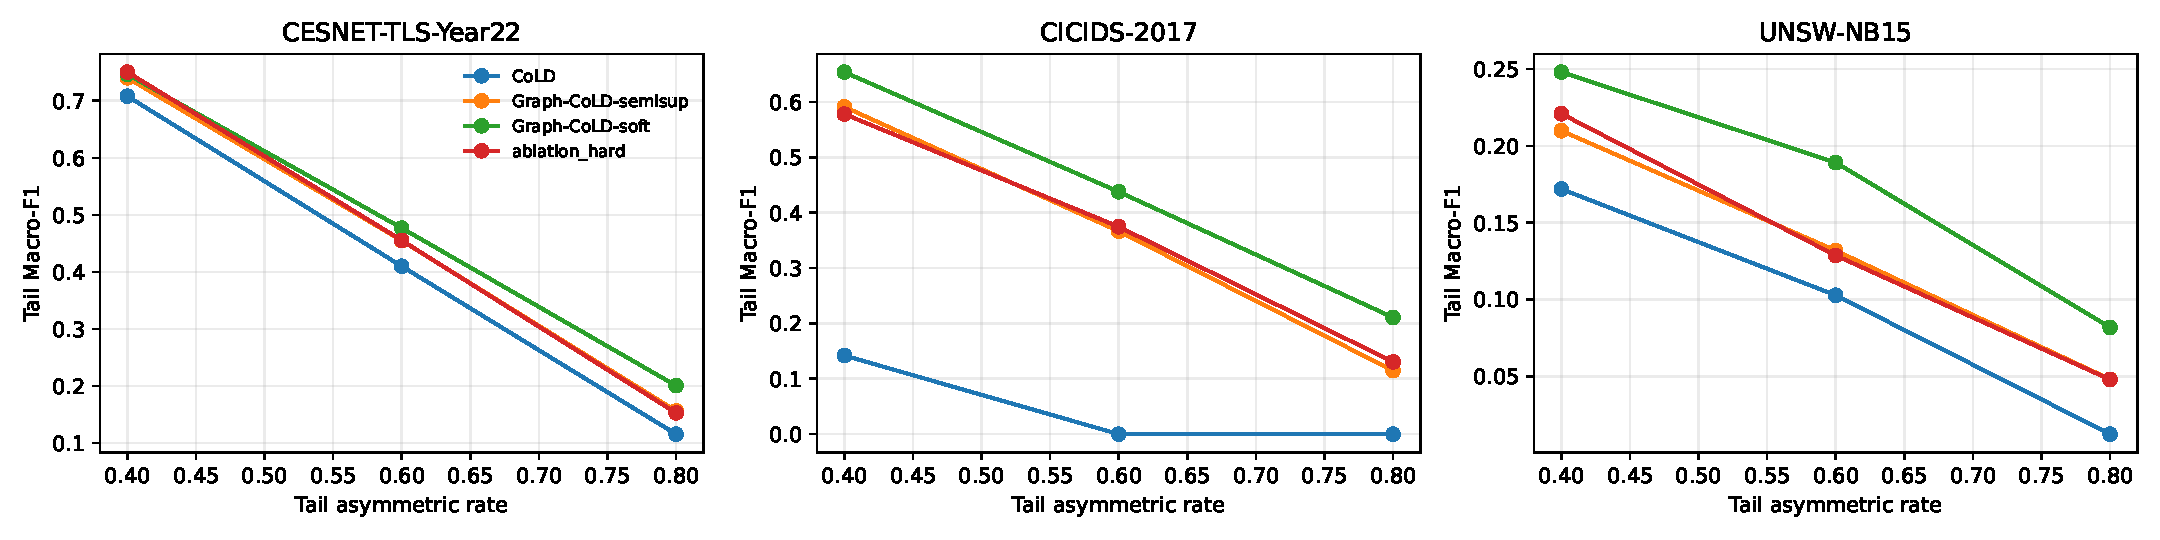
\includegraphics[width=0.98\linewidth]{fig_p2f_tail_powered.pdf}
\caption{Tail-class Macro-F1 of evidence-preserving soft weighting vs.\ hard
deletion across asymmetric noise rates. The gain is small but consistent and
significant on all three datasets.}
\label{fig:tail}
\end{figure}

We stress an honesty point. An earlier ``rare-evidence recovery rate'' that counted
a sample as recovered whenever it was \emph{retained} was tautological. We redefine
recovery to require correct downstream classification; hard deletion is then no
longer automatically zero. Because soft retention still scores near-ceiling on
this diagnostic,\footnote{The secondary diagnostic values and its definition are
reported in \texttt{tables/table\_p2f\_summary.csv} and
\texttt{reports/p2f\_tighten.md}.} we rely solely on test-set tail-F1 for all
headline comparisons.

\subsection{RQ3: A leakage audit prevents inflated claims}
\label{sec:res-leak}
Our initial pipeline reported a $\sim\!28$-point CICIDS advantage with a curve that
barely degraded under $60\%$ noise—implausible for a denoiser. Auditing revealed
that CICIDS-2017 contains $152{,}201/630{,}399$ ($\approx24\%$) exact-duplicate
training rows, and that any clean-label signal leaking into the evidence/graph
construction inflates results. We verified zero train/test edge crossings, removed
exact and near-duplicate edges, and eliminated the clean-label paths (enforced by a
regression test). The apparent advantage collapses to $+6.7$ points on CICIDS,
$+0.3$ on CESNET, and a slight $-1.3$ on UNSW in the audited comparison
(\texttt{reports/p2c\_leakage\_audit.md}). We report this because graph denoising
in security is unusually susceptible to such inflation.

\subsection{RQ4: Graph informativeness predicts when the method helps}
\label{sec:res-info}
A per-dataset neighborhood-homophily / view-coverage diagnostic correlates with
Graph-CoLD's margin: CICIDS (rich host/IP/temporal views) shows the largest gain,
CESNET sits near a performance ceiling, and UNSW (temporal/process only) shows the
smallest—occasionally negative—margin
(Figure~\ref{fig:info}, \url{tables/table_p2d_graph_informativeness.csv}).
This turns the UNSW result into an informative boundary condition rather than a
failure: when views lack structural signal, the graph diagnostic adds little.

\begin{figure}[t]
\centering
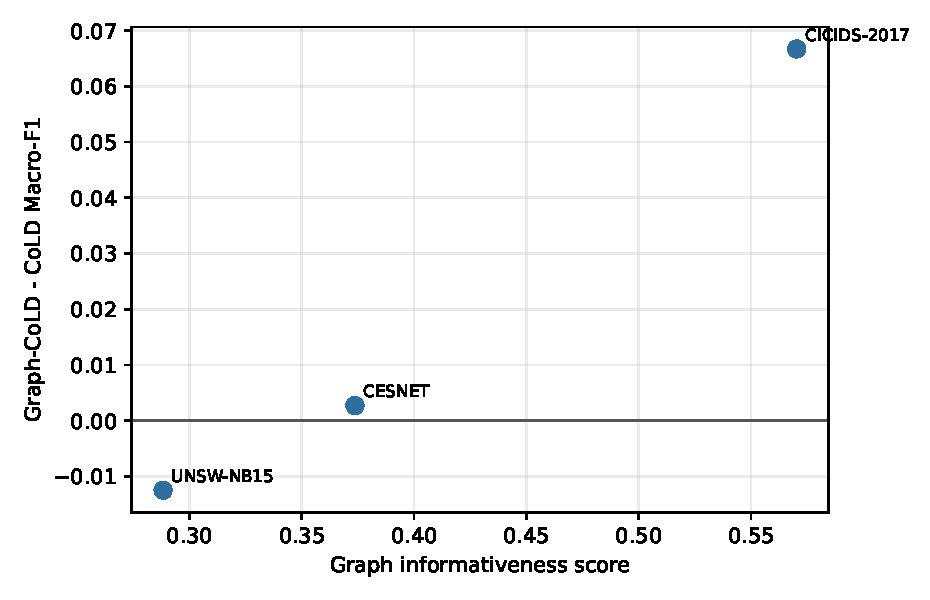
\includegraphics[width=0.9\linewidth]{fig_p2c_informativeness_margin.pdf}
\caption{Graph informativeness vs.\ Graph-CoLD margin over CoLD. Higher
neighborhood homophily and view coverage predict larger gains.}
\label{fig:info}
\end{figure}

\subsection{RQ5: Cost}
Graph-CoLD's overhead is moderate: mean runtime is comparable to CoLD and memory
is lower than the strong purification baselines. Evidence preservation adds
negligible cost over hard deletion because it changes only the training weights.

\section{Discussion}
\label{sec:discuss}
% <<P4-DISCUSSION>>
% BLOCK D -> <<P4-DISCUSSION>>

\subsection{Discussion}

From an operational perspective, Graph-CoLD is most suitable for SOC scenarios
where multiple telemetry sources provide partially consistent evidence. Examples
include environments where host relationships, communication patterns, and
temporal behaviors jointly describe security events. In such settings, a
suspicious sample does not necessarily indicate useless information. A rare
attack instance may appear inconsistent because it represents an emerging
technique rather than because it is incorrectly labeled.

However, the results also demonstrate clear boundaries. When available views
are weak or incomplete, graph structure provides limited additional information.
The UNSW-NB15 results illustrate this condition: without sufficiently
informative relational views, graph-based diagnostics cannot reliably create
additional evidence. Similarly, datasets operating near a performance ceiling,
such as CESNET-TLS-Year22 under the evaluated protocol, naturally limit the
observable improvement.

A key methodological decision in this work is the avoidance of unfair
state-of-the-art comparisons. Earlier experiments included additional
purification and robust-training variants. However, these variants were not all
reimplemented under the final leakage-audited protocol. Mixing results obtained
under different data-cleaning, duplication-removal, and evaluation settings
would create an unreliable comparison. Therefore, the final evaluation uses
aligned baselines with identical data contracts, representation settings, and
statistical protocols. A comprehensive comparison with all previous methods
requires faithful implementations or official code under a unified evaluation
framework.

The leakage audit provides a broader methodological lesson for graph-based
security machine learning. Graph models can unintentionally exploit duplicated
records, cross-split connections, or hidden clean-label information. Such
effects may produce impressive but misleading improvements. Therefore, graph
security studies should explicitly verify data separation, graph construction
constraints, and label independence before reporting performance gains.

Future work should extend Graph-CoLD toward streaming SOC environments,
full-archive evaluation, analyst-in-the-loop validation, and broader
cross-domain benchmark comparisons. These extensions are necessary to determine
whether evidence-preserving denoising remains effective when labels arrive
continuously and attack distributions evolve over time.
The results support a bounded but useful claim. A label-space graph diagnostic
modestly improves noisy-label IDS over CoLD where views are informative, and—more
distinctively—evidence-preserving weighting protects rare-attack evidence that
hard deletion discards, improving tail-class detection under high asymmetric noise
at no aggregate cost. In SOC terms, this matters precisely for the samples an
analyst cannot afford to lose: rare or emerging attacks whose labels are most
likely to be noisy. We deliberately avoid two overclaims that our own experiments
do not support: a universal accuracy advantage (the aggregate gain is modest and
largely from the graph, not the weighting) and a ranking advantage (Graph-CoLD
ties strong peers on top-$K$ precision).

\section{Threats to Validity}
\label{sec:threats}
\emph{Internal.} The evaluation uses deterministic audit windows for tractability;
absolute Macro-F1 is therefore lower than full-archive runs, though the paired,
seed-controlled comparisons are the object of inference. MCRe and MORSE pass a
clean-label sanity floor but degrade on high-noise tabular settings more than in
their original domains; we report this caveat rather than a possibly unfaithful
number (\texttt{reports/p2b\_baseline\_fidelity.md}).
\emph{Construct.} The rare-evidence-recovery diagnostic, even after correction,
saturates for soft retention; we therefore headline test-set tail-F1.
\emph{External.} CICIDS-2017, CESNET-TLS-Year22, and UNSW-NB15 are useful
benchmarks but not complete SOC deployments; the priority score is evaluated by
proxy, not an analyst study. The two-dataset lock recorded in the D9 submission
audit was an intermediate checkpoint; the authoritative final scope is the
three-dataset P2f clean de-oracled protocol.

\section{Limitations}
\label{sec:limits}
MALTLS-22 and OpTC are not evaluated (no verified license/provenance path).
Process and threat-intelligence views are disabled where fields are absent. The
aggregate accuracy contribution is modest and dataset-dependent; the distinctive
contribution is rare-class evidence preservation. Full-archive and streaming
evaluations are left to future work.

\section{Conclusion}
\label{sec:conclusion}
We revisited collaborative label denoising for intrusion detection and asked, with
unusual auditing discipline, whether a multi-view label-space graph diagnostic and
evidence-preserving weighting improve robustness. The honest answer is targeted:
the graph diagnostic gives a modest, informativeness-dependent accuracy gain over
CoLD, and evidence-preserving weighting significantly improves rare-attack tail-F1
over hard deletion under high asymmetric noise at no aggregate cost across three
real datasets. Alongside, we
contribute a leakage audit and a graph-informativeness diagnostic that together
explain when—and when not—graph denoising helps. We hope the audit is as useful to
the community as the method.

%% ------------------------------------------------------------------
\begin{thebibliography}{99}
\bibitem{yang2026cold} S. Yang, X. Zheng, J. Li, J. Xu, E. C. H. Ngai,
``CoLD: Collaborative label denoising framework for network intrusion detection,''
in \emph{Proc. Network and Distributed System Security (NDSS) Symposium}, 2026,
to appear. Available: \url{https://dx.doi.org/10.14722/ndss.2026.231950}
\bibitem{arp2022dodont} D. Arp, et al., Dos and don'ts of machine learning in
computer security, in: USENIX Security Symposium, 2022, pp. 3971--3988.
\bibitem{song2022survey} H. Song, M. Kim, D. Park, Y. Shin, J.-G. Lee,
Learning from noisy labels with deep neural networks: A survey,
IEEE TNNLS 34 (11) (2022) 8135--8153.
\bibitem{patrini2017making} G. Patrini, A. Rozza, A. K. Menon, R. Nock, L. Qu,
Making deep neural networks robust to label noise: A loss correction approach,
in: CVPR, 2017, pp. 1944--1952.
\bibitem{han2018coteaching} B. Han, et al., Co-teaching: Robust training of deep
neural networks with extremely noisy labels, in: NeurIPS, 2018, pp. 8535--8545.
\bibitem{yu2019coteachingplus} X. Yu, et al., How does disagreement help
generalization against label corruption?, in: ICML, 2019, pp. 7164--7173.
\bibitem{malach2017decoupling} E. Malach, S. Shalev-Shwartz, Decoupling ``when to
update'' from ``how to update'', in: NeurIPS, 2017, pp. 960--970.
\bibitem{li2020dividemix} J. Li, R. Socher, S. C. H. Hoi, DivideMix: Learning with
noisy labels as semi-supervised learning, in: ICLR, 2020.
\bibitem{northcutt2021confident} C. G. Northcutt, L. Jiang, I. L. Chuang,
Confident learning: Estimating uncertainty in dataset labels,
JAIR 70 (2021) 1373--1411.
\bibitem{kim2021fine} T. Kim, J. Ko, J. Choi, S.-Y. Yun, FINE samples for learning
with noisy labels, in: NeurIPS, 2021, pp. 24137--24149.
\bibitem{wu2023morse} X. Wu, W. Guo, J. Yan, B. Coskun, X. Xing, From grim reality
to practical solution: Malware classification in real-world noise, in: IEEE S\&P,
2023, pp. 2602--2619.
\bibitem{yuan2023mcre} Q. Yuan, G. Gou, Y. Zhu, Y. Zhu, G. Xiong, Y. Wang,
MCRe: A unified framework for handling malicious traffic with noise labels,
IEEE Transactions on Information Forensics and Security, 2023.
\bibitem{kipf2017gcn} T. N. Kipf, M. Welling, Semi-supervised classification with
graph convolutional networks, in: ICLR, 2017.
\bibitem{velickovic2018gat} P. Veli\v{c}kovi\'c, et al., Graph attention networks,
in: ICLR, 2018.
\bibitem{hamilton2017graphsage} W. L. Hamilton, R. Ying, J. Leskovec, Inductive
representation learning on large graphs, in: NeurIPS, 2017.
\bibitem{hu2020hgt} Z. Hu, Y. Dong, K. Wang, Y. Sun, Heterogeneous graph
transformer, in: The Web Conference (WWW), 2020, pp. 2704--2710.
\bibitem{chen2020simclr} T. Chen, S. Kornblith, M. Norouzi, G. Hinton, A simple
framework for contrastive learning of visual representations, in: ICML, 2020,
pp. 1597--1607.
\bibitem{rehman2024flash} M. U. Rehman, H. Ahmadi, W. U. Hassan, Flash: A
comprehensive approach to intrusion detection via provenance graph representation
learning, in: IEEE S\&P, 2024, pp. 3552--3570.
\bibitem{xu2024argus} J. Xu, X. Shu, Z. Li, Understanding and bridging the gap
between unsupervised network representation learning and security analytics, in:
IEEE S\&P, 2024, pp. 3590--3608.
\bibitem{yang2021cade} L. Yang, et al., CADE: Detecting and explaining concept
drift samples for security applications, in: USENIX Security Symposium, 2021,
pp. 2327--2344.
\bibitem{vaarandi2024nids} R. Vaarandi, A. Guerra-Manzanares, Network IDS alert
classification with active learning techniques, Journal of Information Security
and Applications 81 (2024) 103687.
\bibitem{chavali2024rlalert} L. Chavali, A. Krishnan, P. Saxena, B. Mitra,
A. Sreevallabh Chivukula, Off-policy actor-critic deep reinforcement learning for
alert prioritization in intrusion detection systems, Computers \& Security 142
(2024) 103854.
\bibitem{sharafaldin2018cicids} I. Sharafaldin, A. H. Lashkari, A. A. Ghorbani,
Toward generating a new intrusion detection dataset and intrusion traffic
characterization, in: ICISSP, 2018, pp. 108--116.
\bibitem{hynek2024cesnet} K. Hynek, J. Luxemburk, J. Pesek, T. Cejka, P. Siska,
CESNET-TLS-Year22: A year-spanning TLS network traffic dataset from backbone
lines, Scientific Data 11 (2024) 1156.
\bibitem{moustafa2015unsw} N. Moustafa, J. Slay, UNSW-NB15: A comprehensive data
set for network intrusion detection systems, in: Military Communications and
Information Systems Conference (MilCIS), 2015, pp. 1--6.
\bibitem{guerra2022datasets} J. L. Guerra, C. Catania, E. Veas, ``Datasets are not
enough: Challenges in labeling network traffic,'' \emph{Computers \& Security} 120
(2022) 102810.
\bibitem{qing2023lowquality} Y. Qing et al., ``Low-quality training data only? A
robust framework for detecting encrypted malicious network traffic,'' arXiv
preprint arXiv:2309.04798, 2023.
\bibitem{zhao2021enhancing} Z. Zhao et al., ``Enhancing robustness of on-line
learning models on highly noisy data,'' IEEE TDSC 18(5) (2021) 2177--2192.
\bibitem{wang2022feco} N. Wang et al., ``FeCo: Boosting intrusion detection
capability in IoT networks via contrastive learning,'' in: IEEE INFOCOM, 2022,
pp. 1409--1418.
\bibitem{yue2022cleid} Y. Yue et al., ``Contrastive learning enhanced intrusion
detection,'' IEEE TNSM 19(4) (2022) 4232--4247.
\bibitem{liu2025deepdrac} Y. Liu et al., ``DeepDRAC: Disposition recommendation
for alert clusters based on security event patterns,'' IEEE TIFS 20 (2025)
6443--6458.
\bibitem{shon2023semisup} H. G. Shon, Y. Lee, M. Yoon, ``Semi-supervised alert
filtering for network security,'' Electronics 12(23) (2023) 4755.
\bibitem{wang2024alertagg} W. Wang et al., ``Transformer-based framework for
alert aggregation and attack prediction in a multi-stage attack,'' \emph{Computers
\& Security} 136 (2024) 103533.
\bibitem{xia2021sample} X. Xia et al., ``Sample selection with uncertainty of
losses for learning with noisy labels,'' arXiv preprint arXiv:2106.00445, 2021.
\bibitem{liu2021metric} C. Liu et al., ``Noise-resistant deep metric learning with
ranking-based instance selection,'' in: CVPR, 2021, pp. 6811--6820.
\bibitem{yang2024recda} S. Yang et al., ``RecDA: Concept drift adaptation with
representation enhancement for network intrusion detection,'' in: ACM SIGKDD,
2024, pp. 3818--3828.
\bibitem{andresini2021insomnia} G. Andresini et al., ``Insomnia: Towards
concept-drift robustness in network intrusion detection,'' in: ACM AISec, 2021,
pp. 111--122.
\bibitem{hynek2024zenodo} K. Hynek et al., CESNET-TLS-Year22 dataset, Zenodo
record 10608607, 2024.
\bibitem{moustafa2016unsw} N. Moustafa, J. Slay, ``The evaluation of network
anomaly detection systems: UNSW-NB15,'' Information Security Journal 25(1--3)
(2016) 18--31.
\end{thebibliography}

\end{document}
